% -*- mode: latex; -*-
\documentclass[sigconf]{acmart}

%%
%% \BibTeX command to typeset BibTeX logo in the docs
\AtBeginDocument{%
  \providecommand\BibTeX{{%
    \normalfont B\kern-0.5em{\scshape i\kern-0.25em b}\kern-0.8em\TeX}}}

%% Rights management information.  This information is sent to you
%% when you complete the rights form.  These commands have SAMPLE
%% values in them; it is your responsibility as an author to replace
%% the commands and values with those provided to you when you
%% complete the rights form.
\setcopyright{acmcopyright}
\copyrightyear{2021}
\acmYear{2021}


%%%%%%%%%%%%%%%%%%%%%%%%%%%%%% Packages %%%%%%%%%%%%%%%%%%%%%%%%%%%%%%%%%%%%%%%%
%%%%%%%%%%%%%%%%%%%%%%%%%%%%%%% Packages %%%%%%%%%%%%%%%%%%%%%%%%%%%%%%%%%%%%%%%
\usepackage{graphicx}
\usepackage{epsfig}
\usepackage{times}
\usepackage[ruled,vlined]{algorithm2e}            %% for algorithms
\usepackage{amsmath}
\usepackage{amsthm}                  %% for theorems and definitions
% \usepackage{amssymb}                 %% for arrows like rightarrowtail
\usepackage{amsfonts}                %% \mathbb
\usepackage{mathtools}               %% for coloneqq and others
\usepackage{cases}                   %% better math brackets
\usepackage{mathpartir}              %%% for inference rules
\usepackage[nolist]{acronym}
\usepackage{hyperref}                %% for auto references
\usepackage{xpunctuate}              %% for punctuation's after macros
% \usepackage{cite}                    %% for bibliography ranges
\usepackage{subcaption}              %% For complex figures with subfigures/subcaptions
\usepackage{wrapfig}                 %% wrapping figures around text
\usepackage{listings}                %% for source code lstlisting
\usepackage{enumitem}                %% For better enumerate environment
\setlist[description]{leftmargin=\parindent,labelindent=\parindent}
\usepackage{caption}
\usepackage{multirow}                %% for multiple rows in tables
\usepackage{tikz}                    %% assertion stack visualization
\usepackage[T1]{fontenc}             %% For escaping special characters in bibtex
\usetikzlibrary{matrix}
\usetikzlibrary{arrows}
\usetikzlibrary{positioning}
\usetikzlibrary{shapes.multipart}
\usetikzlibrary{automata}
\usetikzlibrary{cd}                  %% for commuting diagrams

\usepackage{lib/paperCommands}

%%%%%%%%%%%%%%%%%%%%%%%%%%%%%%% End Packages %%%%%%%%%%%%%%%%%%%%%%%%%%%%%%%%%%


%%%%%%%%%%%%%%%%%%%%%%%%%%%%%%% Packages Configs %%%%%%%%%%%%%%%%%%%%%%%%%%%%%%%%%%
\graphicspath{ {./Figures/} }
\raggedbottom

\theoremstyle{definition}
\newtheorem{theorem}{Theorem}[section]
\newtheorem{definition}{Definition}[section]
\newtheorem{corollary}{Corollary}[theorem]
\newtheorem{lemma}[theorem]{Lemma}
\newtheorem*{analysis}{Analysis}

\DeclareMathOperator*{\minimize}{minimize}

\SetKwInOut{Input}{Input}                % Set the Input
\SetKwInOut{Output}{Output}              % set the Output

\lstdefinelanguage{SMTLIB}{
    alsoletter={\-},
    morekeywords={push,pop,assert,check-sat,declare,const,define,fun,and,or,not,check,sat,get,model,reset},
    morecomment=[l]{;},
    morestring=[b]{"},
    sensitive=false,
}

\lstset{
  frame=top,frame=bottom,
  basicstyle=\linespread{.99}\small\normalfont\sffamily,    % the size of the fonts that are used for the code
  commentstyle=\color{Gray},
  keywordstyle=\color{NavyBlue},
  stepnumber=1,                           % the step between two line-numbers. If it is 1 each line will be numbered
  numbersep=10pt,                         % how far the line-numbers are from the code
  tabsize=2,                              % tab size in blank spaces
  extendedchars=true,                     %
  breaklines=true,                        % sets automatic line breaking
  captionpos=t,                           % sets the caption-position to top
  mathescape=true,
  showstringspaces=false,
  escapeinside={(*@}{@*)},%
  literate = {-}{-}1
 }

\newcommand{\lstvdots}{%
  \raisebox{-1pt}[0pt][0pt]{%
    \scalebox{0.7}{\ensuremath{\vdots}}}%
  \hspace{-1.5pt}}

\reversemarginpar
%%%% new environment for sub-proofs
\newenvironment{subproof}[1][\proofname]{%
  \renewcommand{\qedsymbol}{\ensuremath{\blacksquare}}%
  \begin{proof}[#1]%
}{%
  \end{proof}%
}

\newenvironment{MAlgorithm}[1][htb]
  {\renewcommand{\algorithmcfname}{M}% Update algorithm name
   \begin{algorithm}[#1]%
  }{\end{algorithm}}

\renewcommand{\sectionautorefname}{Section }
%%%%%%%%%%%%%%%%%%%%%%%%%%%%%%% End Packages Configs %%%%%%%%%%%%%%%%%%%%%%%%%%%%%%



%%%%%%%%%%%%%%%%%%%%%%%%%%%%%% Kick Off %%%%%%%%%%%%%%%%%%%%%%%%%%%%%%%%%%%%%%%%
\begin{document}

\title{The Name of the Title is Hope}

\author{Colin Shea-Blymyer}
\email{sheablyc@oregonstate.edu}
\affiliation{%
  \institution{Oregon State University}
  \city{Corvallis}
  \state{Oregon}
  \country{USA}
}
\author{Jeffrey M. Young}
\email{youngjef@oregonstate.edu}
\affiliation{%
  \institution{Oregon State University}
  \city{Corvallis}
  \state{Oregon}
  \country{USA}
}

\renewcommand{\shortauthors}{Shea-Blymyer and Young.}

%%
%% The abstract is a short summary of the work to be presented in the
%% article.
\begin{abstract}
  The minimum feedback arc set problem is the problem of finding the least amount
of edges in a directed, cyclic, graph, such that if these edges are removed a
directed, acyclic graph results. There are exists several classic and
approximate methods to solve the minimum feedback arc set problem. In this
study, we explore the novel use of \ac{smt} solvers to solve the minimum
feedback arc set problem. With an \ac{smt} solver, we hypothesize that not only
is an effective encoding possible, but by employing advanced features of
\ac{smt} solvers, such as incrementality and unsatisfiable cores, we can provide
users with decision points to give users the ability to pause the solution
routine, resample particular edges, alter the problem or inspect intermediate
results. Our results are negative. We find an effective \ac{smt} encoding for
the minimum feedback arc set problem but the encoding produces \ac{smt} problems
that in practice are unreasonably slow. Similarly, we find that to make
effective use of incrementality and unsatisfiable cores, one would require
information which is itself an instance of the minimum feedback arc set, and
thus these features are ill suited to this problem domain.


%%% Local Variables:
%%% mode: latex
%%% TeX-master: "../main"
%%% End:
\end{abstract}

%%
%% Keywords. The author(s) should pick words that accurately describe
%% the work being presented. Separate the keywords with commas.
\keywords{datasets, neural networks, gaze detection, text tagging}

% \begin{teaserfigure}
%   \includegraphics[width=\textwidth]{round_robin_graph}
%   \caption{Seattle Mariners at Spring Training, 2010.}
%   \Description{Enjoying the baseball game from the third-base
%   seats. Ichiro Suzuki preparing to bat.}
%   \label{fig:teaser}
% \end{teaserfigure}

%% information and builds the first part of the formatted document.
\maketitle


\section{Introduction}
\label{section:introduction}%

Your introduced $\ldots{}$



%%% Local Variables:
%%% mode: latex
%%% TeX-master: "../main"
%%% End:

\section{Background}
\label{section:background}

In this section, we provide background on the minimum feedback arc set problem,
incremental \ac{sat} and \ac{smt} solving, and unsatisfiable cores. We begin
with preliminaries on graphs and feedback arc sets.

On a directed graph \graph{G}{V}{E} a \emph{feedback arc set} \fas{S} is a set
of edges in $\kf{E}$, such that removing them from the graph $\kf{G}$ results in
an acyclic graph. The minimum feedback arc set problem finds the
\optimal{\fas{S}} of the minimum size. For weighted graphs, one might desire
\optimal{\fas{S}} to have the minimum total weight of any \fas{S}. Finding this
\optimal{\fas{S}} is the minimum weighted feedback arc set problem.

\NOTE{Hi Mike! This is a special note environment just for you. From this point
  we plan on giving an overview of the necessary interface for sat and smt
  solving. We're planning on adapting this from Jeff's PhD thesis, so it won't
  be from whole cloth.}



%%% Local Variables:
%%% mode: latex
%%% TeX-master: "../main"
%%% End:

\section{Gadgets}
\label{section:gadgets}
%
\begin{figure}[h]
  \centering
  \begin{lstlisting}[language=python,caption={Cycle check gadget. \texttt{v\_from}
  and \texttt{v\_to} are symbolic variables in the solver. \texttt{name} is the constraint
  label in the solver. The cycle check replaces each edge with the constraint
  that previous vertices must be a lesser integer value than future vertices}]
  def cycle_check(solver,v_from,v_to,name):
      solver.assert_and_track(v_from < v_to, name)
  \end{lstlisting}
\end{figure}

Our approach is to translate an exact integer programming method by
\citet{alietall} to an \ac{smt} problem. The translation to an \ac{smt} problem
is straightforward, requiring no changes from linear program encoding to an
\ac{smt} encoding.

To find the minimum feedback arc set of a graph \grph{G}, the method requires a
cycle matrix, \cmatrix{i}{j}. The cycle matrix tracks which edges are in which
cycles in the graph. For some edge \symEdge{j}, if \symEdge{j} participates in
cycle $\kf{i}$ then \cmatrix{i}{j} = 1 otherwise \cmatrix{i}{j} = 0, indicating
that \symEdge{j} \emph{does not} participate in the $\kf{i}$th cycle. For
example, consider the edge \edge{B}{D} from \autoref{fig:three-cycle} and assume
\edge{B}{D} has edge ID $\kf{j} = 3$, if the 0th cycle in
\autoref{fig:three-cycle} is composed of edges: \edge{A}{B}, \edge{B}{C}, and
\edge{C}{A}, then \cmatrix{0}{3} = 0. Similarly, assuming \edge{A}{B} has edge
ID $\kf{j} = 0$, then \cmatrix{0}{0} = 1 because \edge{A}{B} participates in
cycle 0.

With the cycle matrix, the method is composed of $\kf{c}$ constraints, where
$\kf{c}$ is the number of cycles and a minimization over the sum of edges. Each
edge, \edge{i}{j} is encoded as a binary integer \ac{smt} variable \symEdge{j},
where $\kf{j}$ is the edge's unique ID. The \ac{smt} variable \symEdge{j} only
ranges from 0 to 1, indicating whether the $\kf{j}$th edge is in the minimum
feedback arc set (\symEdge{j} = 1) or not (\symEdge{j} = 0). We express the
constraints in the following equations:
%
\begin{equation}
  \label{one}
 \minimize \sum_{j=1}^{\magnitude{E}} \symEdge{j}
\end{equation}
%
\begin{equation}
  \label{two}
  (\sum_{j=1}^{\magnitude{E}} \cmatrix{i}{j} \symEdge{j}) \ge 1, \, \text{for each } i = 0, 1, 2 \dots{}, c
\end{equation}

Conceptually, \autoref{one} requires the \ac{smt} solver to consider all edges
in the graph \grph{G} and find the smallest number of edges which compose a
feedback arc set. The encoding of a feedback arc set occurs in \autoref{two}.
With the constraint $\sum (\dots) \ge 1$ for the $\kf{i}$th cycle, \autoref{two}
states that for each cycle in the graph \grph{G} pick one or more edges. By
$\sum (\cmatrix{i}{j} \symEdge{j}) \ge 1$, \autoref{two} forces the \ac{smt}
solver to consider edges that occur in most cycles. The logic is easiest to
observe with an example, consider the graph shown in \autoref{fig:three-cycle},
with the edge and cycle IDs shown in \autoref{table}:
%
\begin{table}
  \begin{subtable}[t]{0.20\textwidth}
  \begin{tabular}{|c c|}
    \hline
    Edge & ID \\ [0.5ex]
    \hline\hline
    \edge{A}{B} & 0 \\
    \edge{B}{C} & 1 \\
    \edge{C}{A} & 2 \\
    \edge{B}{D} & 3 \\
    \edge{D}{E} & 4 \\
    \edge{E}{F} & 5 \\
    \edge{F}{C} & 6 \\
    \edge{F}{D} & 7 \\ [1ex]
    \hline
  \end{tabular}%
\end{subtable}%
~
\begin{subtable}[t]{0.80\textwidth}
  \begin{tabular}{|c c|}
    \hline
    Cycle & Cycle edges \\ [0.5ex]
    \hline\hline
    0 & \edge{A}{B} $\rightarrow$ \edge{B}{C} $\rightarrow$ \edge{C}{A} \\[0.5ex]
    1 & \edge{D}{E} $\rightarrow$ \edge{E}{F} $\rightarrow$ \edge{F}{D} \\[0.5ex]
    \multirow{2}{2em}{\centering 2} & \edge{A}{B} $\rightarrow$ \edge{B}{D} $\rightarrow$ \edge{D}{E} \\
                         & \edge{E}{F} $\rightarrow$ \edge{F}{C} $\rightarrow$ \edge{C}{A} \\
    \hline
  \end{tabular}%
\end{subtable}
\caption{Table of Edge IDs and Cycle IDs for \autoref{fig:three-cycle}}%
\label{table}%
\end{table}
%
For this graph, the constraints generated by \autoref{two} would be:
%
\begin{align*}
  1\symEdge{0} + 1\symEdge{1} + 1\symEdge{2} + 0\symEdge{3} + 0\symEdge{4} + 0\symEdge{5} + 0\symEdge{6} + 0\symEdge{7} \ge 1 & \qquad \text{Cycle 0} \\
  0\symEdge{0} + 0\symEdge{1} + 0\symEdge{2} + 0\symEdge{3} + 1\symEdge{4} + 1\symEdge{5} + 0\symEdge{6} + 1\symEdge{7} \ge 1 & \qquad \text{Cycle 1} \\
  1\symEdge{0} + 0\symEdge{1} + 1\symEdge{2} + 1\symEdge{3} + 1\symEdge{4} + 1\symEdge{5} + 1\symEdge{6} + 0\symEdge{7} \ge 1 & \qquad \text{Cycle 2}
\end{align*}

Where we see the edge \symEdge{0} (edge \edge{A}{B}) occurs in cycles 0, and 2
(as \cmatrix{0}{0} and \cmatrix{2}{0} = 1). Therefore, the easiest way for the
\ac{smt} solver to satisfy these constraints \emph{and} the minimization
constraint is to set $\symEdge{0} = 1$. However, doing so will not satisfy the
cycle constraints for cycle 1, thus the solver must pick either \symEdge{4}
(\edge{D}{E}), \symEdge{5} (\edge{E}{F}), or \symEdge{7} (\edge{F}{C}). Again
the simplest path is to pick \symEdge{4}, or \symEdge{5} as setting these
variables to 1 satisfies more than one constraint. Thus, we see that by this
encoding the \ac{smt} solver is forced to minimize the number of edges to pick,
and therefore maximize the number of cycle constraints satisfied by setting a
given edge to 1, which corresponds to finding the minimum feedback arc set of a
graph.

%%% Local Variables:
%%% mode: latex
%%% TeX-master: "../main"
%%% End:

\section{Case Studies}
\label{section:case-studies}
%
To evaluate this approach, we construct a prototype \ac{smt}-enabled algorithm
and assess the prototype on Erd\H{o}s-R\'{e}nyi graphs. Erd\H{o}s-R\'{e}nyi
graphs are generated according to two parameters: $\kf{p}$, a metric of
connectedness for the graph, and $\kf{k}$ is the number of vertices in the
graph.

With these parameters we employ random generation to construct sample graphs. We
are interested in the individual effect $\kf{k}$ and $\kf{p}$ have on runtime,
in addition to the interactions effects between each parameter. Consider the
case where $\kf{p}$ and $\kf{k}$ are left unbound, yet $\kf{s}$ is set to 1.
This is the specific case where solving the minimum weighted feedback arc set
problem solves the minimum feedback arc set problem. Thus, by setting $\kf{s}$
to 1 we generate graphs to solve the minimum feedback arc set problem. Consider
the case where $\kf{s}$ is larger than one. In this case, edges must possess
positive weights and the weighted minimum feedback arc set may be different than
the minimum feedback arc set.

We provide the complete prototype implementation in
\autoref{appendix:source-code-listings}. To ensure correctness we compared
results from the \ac{smt} routine to a built in method in the python library
\lstinline{igraph} which finds the minimum feedback arc set. We observed no
differences between both methods.


%%% Local Variables:
%%% mode: latex
%%% TeX-master: "../main"
%%% End:

\section{Results and Discussion}
\label{section:results-and-discussion}

It was good enough to graduate

\begin{figure*}[t]
    \centering
    \includegraphics[width=1\textwidth]{latex/Figures/big_ol_cliff.pdf}
    \caption{A three cycle graph which demonstrates that greedily selecting the
      minimum weighted edge will not provide the minimum feedback arc set.}%
    \label{fig:three-cycle}
\end{figure*}%

%%% Local Variables:
%%% mode: latex
%%% TeX-master: "../main"
%%% End:


\bibliographystyle{ACM-Reference-Format}
\bibliography{sample-base}


%% If your work has an appendix, this is the place to put it.
% \appendix



\end{document}
\endinput
